\section{One-Body Spectral Function and Self-Energy}

The low-energy spectroscopic factors for the one-nucleon removal are obtained
from the one-hole spectral function (\ref{eq:OHSF})
%
\begin{equation}
		S_h(\alpha,\omega)
	=
		\sum_n
		\left|
			\ME< \Psi^{A-1}_n | \Oa{\alpha} | \Psi^A_0 >
		\right|^2
	\;
		\delta\left(\omega - (\EnulA - E^{n,A-1})\right)
	\;.
	\label{eqbis:OHSF}
	\end{equation}
%
As was shown in chapter~\ref{chap:GREEN}, these spectroscopic factors 
correspond to the
residues of the diagonal elements of the one-body Green's function 
(\ref{eq:g1}), which is obtained by solving the Dyson equation 
(\ref{eq:DysonE})
%
	\begin{equation}
		g_{\alpha\beta}(\omega)
	=
		g^0_{\alpha\beta}(\omega)
	+
		\sum_{\gamma\delta}
		g^0_{\alpha\gamma}(\omega)
		\Sigma^\ast_{\gamma\delta}(\omega)
		g^{\phantom{0}}_{\delta\beta}(\omega)
	\;.
	\label{eqbis:DysonE}
	\end{equation}
%
In a calculation within a finite model space it appears that the one-body
propagator is, in a good approximation, diagonal. 
For simplicity, the self-energy
and the propagators are assumed to be diagonal below.
The spectroscopic factors are obtained by means of  
the normalization condition (\ref{eq:DysNorm})
%
	\begin{equation}
		\left|
		\ME<\Psi^{m,A-1}| \Oa{\alpha} | \Psi^A_0 >
		\right|^2
	=
		\left(
			1
		-
			\frac{
				{\rm d} \Sigma_\alpha^\ast(\omega)
			}{
				{\rm d} \omega
			}
		\right)^{-1}_{\omega=\EnulA - E^{m,A-1}}
	\label{eq:sfNorm}
	\;.
	\end{equation}
%
The Dyson equation can not be solved without an appropriate approximation for
the self-energy $\Sigma^\ast$. In the calculations below the approximation 
for the self-energy includes the diagrams of fig.~\ref{fig:selfenergy}.
%%%%%%%%%%%%%%
\begin{figure}
\centerline{
\cntrbox{3cm}{2cm}{ \epsfig{ file=figures/selfenergy/sig_HF.ps, width=2cm } }
\cntrbox{3cm}{2cm}{ \epsfig{ file=figures/selfenergy/pphtda.ps, width=2cm } }
\cntrbox{3cm}{2cm}{ \epsfig{ file=figures/selfenergy/hhptda.ps, width=2cm } }
}
\caption[]{Graphical representation of some contributions to the irreducible 
self-energy $\Sigma^\ast$ that appear in the Dyson equation (\ref{eq:Dyson}).
The thick lines indicate single-particle propagator $g$, that is 
the solution of the Dyson equation. The wiggly lines denote the G-matrix
interaction. The first diagram is the 
Hartree-Fock contribution (\ref{eq:SigHFe}), the second and third diagram 
include two-particle-one-hole and two-hole-one-particle interactions in 
Tamm-Dancoff approximation, \cf\ (\ref{eq:SigTDA}). These diagrams define 
the approximation for the self-energy used in this chapter.
\label{fig:selfenergy}
}
\end{figure}
%%%%%%%%%%%%%%
In the Hartree-Fock (HF)
 diagram the energy-dependence of the  G-matrix simulates the effect 
of short-range correlations at low energy; the 2p1h and 2h1p propagator 
diagrams should 
account for the fragmentation of strength at low energy due to 
long-range correlations. This 2p1hTDA self-energy has been studied in 
ref.~\cite{RGAD95}, in which it is noted that a logical extension of this 
formalism in the form of an RPA like series for the 2p1h propagator is not
straightforward.

\subsection{Energy Dependence of (Brueckner)HF Self-Energy}
The contribution to the irreducible self-energy of first order in the G-matrix,
depicted in the Hartree-Fock diagram of fig.~\ref{fig:selfenergy}, is 
given by 
%
	\begin{eqnarray}
		\Sigma^{HF}_{\alpha\beta}(\omega)
	&=&
		i
		\sum_{\gamma\delta}
		\int \frac{{\rm d}\omega' }{ 2\pi }
	\;
		{\rm G}_{\alpha\gamma\beta\delta}( \omega+\omega' )
	\;
		g_{\gamma\delta}( \omega' )
	\label{eq:SigHFe}
	\;,
	\end{eqnarray}
%
where the proper energy-dependence of G is taken into account.
It appears that, within the chosen model space, the off-diagonal elements of 
$\Sigma^{HF}$ (\ref{eq:SigHFe}), which would give rise to mixing of orbits 
with different radial oscillator quantum numbers, are unimportant. Therefore 
we shall henceforth formulate everything in diagonal form.
In the case of an energy-dependent interaction (G-matrix)
the single-particle energies in the HF propagator,
of which only the diagonal contributions are given here,
\cf\ (\ref{eq:g10}), also become energy-dependent
%
	\begin{equation}
		g^{HF}_{\alpha}(\omega)
	=
		\left[
		\frac{
			\theta( \alpha - F )
		}{ \omega - \varepsilon^{HF}_\alpha(\omega) +i \eta }
	+
		\frac{
			\theta(  F - \alpha )
		}{ \omega - \varepsilon^{HF}_\alpha(\omega) -i \eta }
		\right]
	\label{eqbis:gHF}
	\;,
	\end{equation}
%
with
%
	\begin{eqnarray}
		\varepsilon^{HF}_\alpha(\omega)
	&=&
			T_{\alpha}
			+
			\Sigma^{HF}_{\alpha}(\omega)
	\nonumber \\
	&=&
			\half \hbar \Omega^2
			\ME< n_\alpha l_\alpha | r^2 | n_\alpha l_\alpha >
			+
			\sum_{\gamma < F}
			{\rm G}_{\alpha\gamma\alpha\gamma}
			(\omega+\varepsilon_\gamma)
	\label{eq:eHFom}
	\;.
	\end{eqnarray}
%
The kinetic energy is equal to 
the potential energy for the diagonal elements shown here, 
because the basis consists of harmonic oscillator states.
The off-diagonal terms of the kinetic energy equal minus the potential energy.
The summation in (\ref{eq:eHFom})
runs over all states below the Fermi level and the 
self-consistency relation 
%
	\begin{equation}
		\omega
	=
		\varepsilon^{HF}_\alpha(\omega)
	\label{eq:omeqeps}
	\end{equation}
%
should be imposed.
The energy-dependence in the range of energies around the Fermi level is very
smooth, so the self-consistent solutions of (\ref{eq:omeqeps}) can be 
obtained by interpolation, see fig.~\ref{fig:Ehf}.
%%%%%%%%%%%%%%
\begin{figure}
\centerline{\epsfig{ file=figures/Ehf.ps, width=12.5cm }}
\caption[]{
Values of the $\varepsilon^{HF}_\alpha$ (\ref{eq:eHFom}) 
for $\omega=-110$, $-70$, $-40$, $-20$ and~$-5$~MeV.
The curves belong to ($\alpha=$)$1s\half$ (circles),
$1p\threehalf$ (squares), $1p\half$ (diamonds) and $1d\sfrac{5}{2}$ (triangles).
Intersection of the interpolated curves with the dotted line 
$\omega=\varepsilon^{HF}_\alpha(\omega)$ yields the solution
of the (\ref{eq:omeqeps}).
\label{fig:Ehf}}
\end{figure}
%%%%%%%%%%%%%%%
If the self-energy is restricted to the HF term only, the slope of the curves 
at the crossing points in fig.~\ref{fig:Ehf} now causes a reduction of pole
strength (\ref{eq:sfNorm}) already in HF approximation. In the present 
calculation this reduction is $5$--$7$ \%. It means that the short-range 
correlations,
treated in Brueckner Hartree-Fock approximation, give rise to a high-energy (and
momentum) tail of the spectral function which is of about the same magnitude,
and is 
invisible in the low-energy spectra. This result is consistent with
the numbers obtained in the direct calculation of ref.~\cite{MPD95}, where 
the focus is on the high-momentum part of the spectral 
function. 


\subsection{Coupling to the 2h1p Propagator}
The fragmentation of the particle removal strength over several states in the 
low-energy domain is caused by the mixing of one-hole with 
two-hole-one-particle (2h1p) configurations. In most previous studies the 
residual interaction between the latter three objects was 
neglected\cite{BRM91} or treated to describe collective states with two of 
them, thereby neglecting the Pauli corrections due to the presence of the 
third object\cite{RAD92}.
Moreover, some of the RPA phonons to which the hole was coupled, became
unstable with the G-matrix interaction and were simply discarded in 
ref~\cite{RAD92}.
For these reasons we wish to treat the mixing of 
two-hole-one-particle configurations explicitly. This is achieved in a 
recent study\cite{RGAD95}
in which the self-energy is expressed using the 2p1h Green's function
%
	\begin{equation}
		iR_{mnl;pqs}(t-t')
	=
		\ME< \Psi_0^A|
		T\left[
			\Oc{l}(t)  \Oa{n}(t)  \Oa{m}(t)
			\Oc{p}(t') \Oc{q}(t') \Oa{s}(t')
		\right]
		|\Psi_0^A>
	\;.
	\label{eq:gR}
	\end{equation}
%
It can be shown\cite{Wi72} that contributions to the self-energy beyond 
the Hartree-Fock term may be expressed as
%
	\begin{equation}
		\Sigma^\ast_{\alpha\beta}(\omega)
	=
		\sum_{mnl; pqs}
		\half
		V_{\alpha lmn}
	\;
		\bar{R}_{mnl;pqs}(\omega)
	\;
		\half
		V_{pq\beta s}
	\label{eq:SigTDA}
	\end{equation}
%
in which $\bar{R}$ is the irreducible version of (\ref{eq:gR}), \ie\
the set of all diagrams, excluding the ones which have only one line at 
an intermediate time. Of course, the infinite series of diagrams for 
$\bar{R}$ must be approximated in some way. 
Collective features of both pp- and ph-correlations can be taken into account 
in Tamm-Dancoff approximation (TDA) by
retaining those diagrams which have just three lines at all times.
Therefore, this approximation was called\cite{RGAD95} the 
`Faddeev' approximation of the 
2p1h-propagator. This approach leads to the 2p1h (2h1p)TDA equation.  
The 2p1hTDA equation is depicted in fig.~\ref{fig:2p1hTDA}.
%%%%%%%%%%%%%
\begin{figure}
\begin{eqnarray}
\lefteqn{
\cntrbox{2cm}{2cm}{\epsfig{figure=figures/2p1hTDA/hhpTDA1.ps, height=2cm}}
=
\cntrbox{2cm}{2cm}{\epsfig{figure=figures/2p1hTDA/hhpTDA2.ps, height=2cm}}
-
\cntrbox{2cm}{2cm}{\epsfig{figure=figures/2p1hTDA/hhpTDA3.ps, height=2cm}}
} && \nonumber \\
&&
+
\cntrbox{2cm}{2cm}{\epsfig{figure=figures/2p1hTDA/hhpTDA4.ps, height=2cm}}
+
\cntrbox{2cm}{2cm}{\epsfig{figure=figures/2p1hTDA/hhpTDA5.ps, height=2cm}}
+
\cntrbox{2cm}{2cm}{\epsfig{figure=figures/2p1hTDA/hhpTDA6.ps, height=2cm}}
\nonumber
\end{eqnarray}
\caption[]{The Tamm-Dancoff approximation for the 2p1h propagator. 
\label{fig:2p1hTDA}}
\end{figure}
%%%%%%%%%%%%%
Technically this equation is solved by treating the full interaction 
among configurations of the 2p1h and 2h1p spaces. By diagonalization the 
Hamiltonian within these spaces one obtains the 2p1h (2h1p) energies as
eigenvalues $\omega^\nu$ and the corresponding amplitudes as the eigenvectors
$b^\nu_{lmn}$ in which the indices $l$, $m$ and $n$ denote the particle and 
hole quantum numbers.
The irreducible propagator $\bar{R}$ is then given  in `Faddeev' 
approximation or 2p1hTDA/2h1pTDA as
%
	\begin{equation}
		\bar{R}_{lmn;pqs}(\omega)
	=
		\sum_\nu
		\frac{
			b^\nu_{lmn}
			b^\nu_{pqs}
		}{
		\omega - \omega^\nu
		}
	\label{eq:Risbb}
	\;.
	\end{equation}
%
